\chapter{Application: Standing}\label{chap:standing}
In this chapter, a bang-bang control law on vertical acceleration is implemented in the momentum-based control framework and tested on NASA's Valkyrie \cite{radford2015valkyrie} humanoid robot. Push recovery is tested while the robot is standing. To measure the improvement in balance control, there is compared with a controller that uses a constant reference height. Additionally, an alternative test method is briefly presented using Boston Dynamics' Atlas humanoid robot.

\section{Method}
As the polynomial trajectories of the previous chapter are constraining the vertical acceleration, these are not used in application. Instead, a bang-bang control law for vertical acceleration is designed, similar to the bang-bang control law for the vertical force constrained capture positions in Chapter \ref{sec:verticalforce}.

The desired \ac{CMP} $\rcmpd$ of Equation \eqref{eq:rcmpd} is constrained to be inside the support polygon. Therefore, it is assumed that the angular momentum rate of change is zero, $\dot{\mathbf{k}}_y=0$ [Nm], and that $\rcmpd$ coincides with a desired \ac{CoP} $\rcopd$. The \ac{CoM} height is initially controlled using the default \ac{CoM} height PD control law of Equation \eqref{eq:defaultheightcontrol}.  While the robot is standing still, the control law controls to the default, nominal height:
\begin{equation}
\ddzd =k_p(z_0-z) - k_d\dot{z},
\end{equation}
where $\ddzd$ is the desired vertical acceleration. 

The bang-bang control law is activated when the use \ac{CoP} is saturated. This the case if the \ac{CoP} is on the polygon edge. Because $\rcopd$ is proportionally controlled to the \ac{ICP} error $\icpe$, the bang-bang controller is activated when the $\icpe$ is larger than a minimum \ac{ICP} error threshold $\icpemin$, which can be used for tuning. Note that for the development of a controller for a standing robot, the initial `bang' is always upward, as $\rcopd$ can be placed in the direction of the \ac{ICP} error. This placement of $\rcopd$ is possible, as the \ac{CoM} is inside the support polygon while the robot is standing.

The first and the second acceleration `bang' of the vertical motion controller are jerk limited, unlike the controller for the vertical force constrained capture positions in Section \ref{sec:verticalforce}. Also, the duration of each `bang' is not predefined, but determined online. Determining the duration online, allows for more control of the vertical dynamics, as the current state can be constantly evaluated on violation of the maximum height constraint. A predefined duration as in Section \ref{sec:verticalforce} does not use any feedback and is strictly feedfoward. In relation to these differences in control design, the following parameters are used:
\begin{itemize}
	%\item $\alpha_{\icpe}^+$: Threshold to turn the controller on $|\icpe|>\alpha_{\icpe}^+$, which for example can be tuned to activate the controller when $\rcmpd$ is near the edge of the polygon. 
	%\item $\alpha_{\icpe}^-$: Threshold to turn the controller off $|\icpe|<\alpha_{\icpe}^-$, when the robot is back to stability.
	\item $\dddot{z}_{max}$: maximum allowed vertical CoM jerk;
	\item $\alpha_{\hat{\ddot{z}}_{c}}$: parameter to scale down expected $\ddot{z}_c$ for the second `bang', due to jerk limits.
\end{itemize}
The control sequence for the vertical motion controller reads as follows. For the first `bang', the desired acceleration is set to $\ddot{z}_d=\ddot{z}_c$. The transition from the first `bang' to the second is if the predicted \ac{CoM} height violates the maximum height constraint $\zmax$. This prediction of violation of the constraint is computed as follows, using a conservation of energy:
\begin{align}
	m\hat{g}z + \sgn(\dot{z})\frac{1}{2}\dot{z}^2>m\hat{g}\zmax,\\
	z + \sgn(\dot{z})\frac{1}{2}\frac{\dot{z}^2}{\hat{g}}>\zmax,
\end{align}
where $\hat{g}$ is the predicted downward acceleration of the second `bang'. Using the acceleration constant $\ddzc$ of the second bang and the scale down parameter $\alpha_{\hat{\ddot{z}}_{c}}$ for the predicted downward acceleration, gives:
\begin{equation}
	z+\sgn(\dot{z})\frac{1}{2}\frac{\dot{z}^2}{\alpha_{\hat{\ddot{z}}_{c}}\ddot{z}_{c}} >\zmax.
\end{equation}
When this condition is met, the second `bang' is activated and $\ddot{z}_d=-\ddot{z}_c$. The second `bang' continues until the vertical velocity changes direction: $\dot{z}<0$. This results in the \ac{CoM} height to be controlled to $\zmax$ until the controller turns off:
\begin{equation}
	\ddot{z}_d = k_p(\zmax-z)-k_d\dot{z}.
\end{equation}
Controlling to $\zmax$ allows the robot to apply more force on the ground, compared to controlling directly to $z_0$ again. The controller turns off if the \ac{ICP} error $\icpe$ is at a small value, a measure for stability. If the controller is turned off, the \ac{CoM} height is controlled to the default height and the reference height is set to $z_r=z_0$. Finally, the rate of $\ddot{z}_d$ is limited with the maximum allowed jerk $\dddot{z}_{max}$ and the desired vertical momentum rate is computed as $\dot{\mathbf{l}}_{d,z}=m\ddot{z}_d$. The desired horizontal linear momentum rate is adjusted for the added vertical acceleration as follows:
\begin{equation}
    \dotldxy= \frac{\cxy-\rcopd}{z}(mg+\dot{\mathbf{l}}_{d,z}).
\end{equation}
In the remainder of this chapter, this control law will be compared with the default, constant height, control law that uses \ac{CoP} only. The two control setups will be referred to as:
\begin{itemize}
\item \textbf{Vertical motion}: the control law presented in this section. Results are depicted in blue, unless stated different.
\item \textbf{Default}: the control law as presented in Section \ref{sec:ihmc}. Results are depicted in black, unless stated different.
\end{itemize}
\section{Results}
Tests are conducted by applying a push at chest height on Valkyrie. The parameters and settings used for the tests on Valkyrie can be found in Appendix \ref{chap:params}. Additionally, some tests are conducted on Atlas. To measure the impulse applied on the robot, a normalized impulse $i$ is used:
\begin{equation}
	i = \frac{\int \fpush d\tpush}{\mrobot},
\end{equation}
where $\fpush$ is the push force and $\mrobot$ the robot mass.
\subsection{Valkyrie Simulation}
For Valkyrie in simulation, the push duration is set to $\tpush=0.15$ [s], as on hardware tests it is found that approximately the same push duration can be applied. The push force profile in simulation is constant. A vertical acceleration constant of $\ddzc=2.4$ [m/s$^2$] and a jerk limit of $\dddot{z}_{max}=80.0$ [m/s$^3$] are used, as this was also found to work well on hardware. A value of $\alpha_{\hat{\ddot{z}}_{c}}=0.4$ is used for the prediction of the vertical \ac{CoM} motion. Valkyrie has a total mass of $\mrobot=127.3$ [kg]. Also, an initial height of $z_0=1.0$ [m] is used and a maximum height of $\zmax=1.065$ [m]. 

\subsubsection{Maximum Recoverable Push} 
A search is used in simulation to find the maximum push force where the robot could still recover from. This search is conducted every $5$ degrees.  In \figref{fig:roundStanding}, a polar plot is shown for the maximum recoverable impulses $i$ for the default setup and the vertical motion controller. A push in the back corresponds with $0$ degrees and a frontal push with $180$ degrees.

The recovery improved when using the vertical motion controller after the default controller in push directions coming from the back or the side of the robot. Remarkably, push recovery is worse for push directions coming from the front of the robot, because, according to the \ac{VHIP} model, the direction of the disturbance should not make a difference. Compared to the default setup, the vertical motion controller recovered of a $9$\% higher impulse for a push direction coming from the back of the robot, a $4$\% higher impulse for a push direction coming from the side and a $7$\% lower impulse for a push direction coming from the front. The improvement in maximum recoverable push is the best for a push coming from the back. Also, it is relatively easy to apply a push in the back on the real robot, compared to other parts of the robot. Valkyrie has a hard, flat back surface, which can handle larger impacts than other body parts. For those reasons, there is chosen to make a deeper evaluation of the specific push direction of $0$ degrees, a back push, in simulation too.
\begin{figure}
\centering
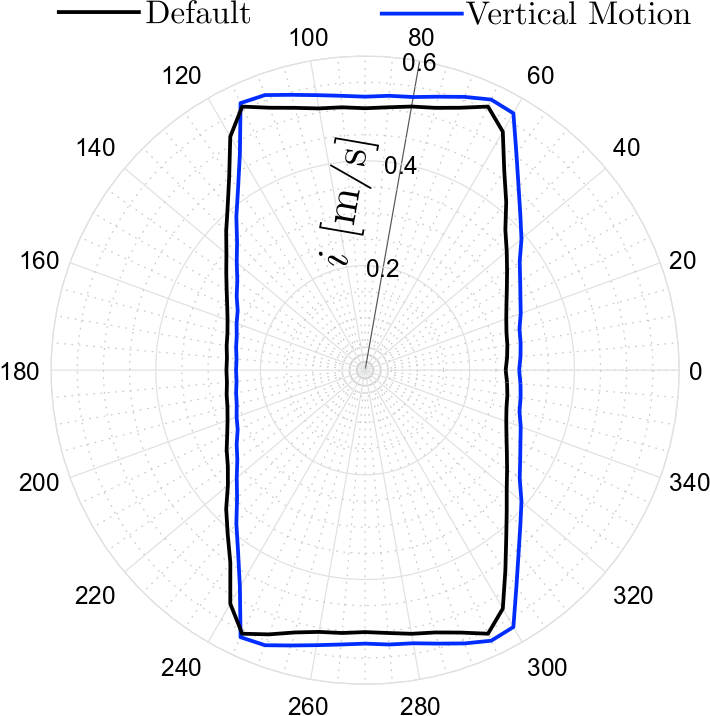
\includegraphics[width=0.6\textwidth]{STYLESTUFF/roundStanding.png}
\caption{Polar plot of maximum recoverable pushes with an increment of $5$ degrees. $0$ degrees is a push from the back. The radius is the normalized impulse $i$. }
\label{fig:roundStanding}
\end{figure}

\subsubsection{Comparison of Equal Push}
To evaluate the responses after a push in the back of the robot, pushes of equal magnitudes are applied on both control setups. In \figref{fig:valcomparephase}, a phase plot is shown for the horizontal \ac{CoM} state in the sagittal plane. One impulse is the maximum recoverable push for the default setup, the other for the vertical motion controller. The area covered by the phase plot is smaller with the vertical motion controller for a push of $i=0.271$ [m/s]. With the larger push of $i=0.295$ [m/s], the default control setup does not manage to stabilize and diverges, while the vertical motion controlled setup recovers.
\begin{figure}
\centering
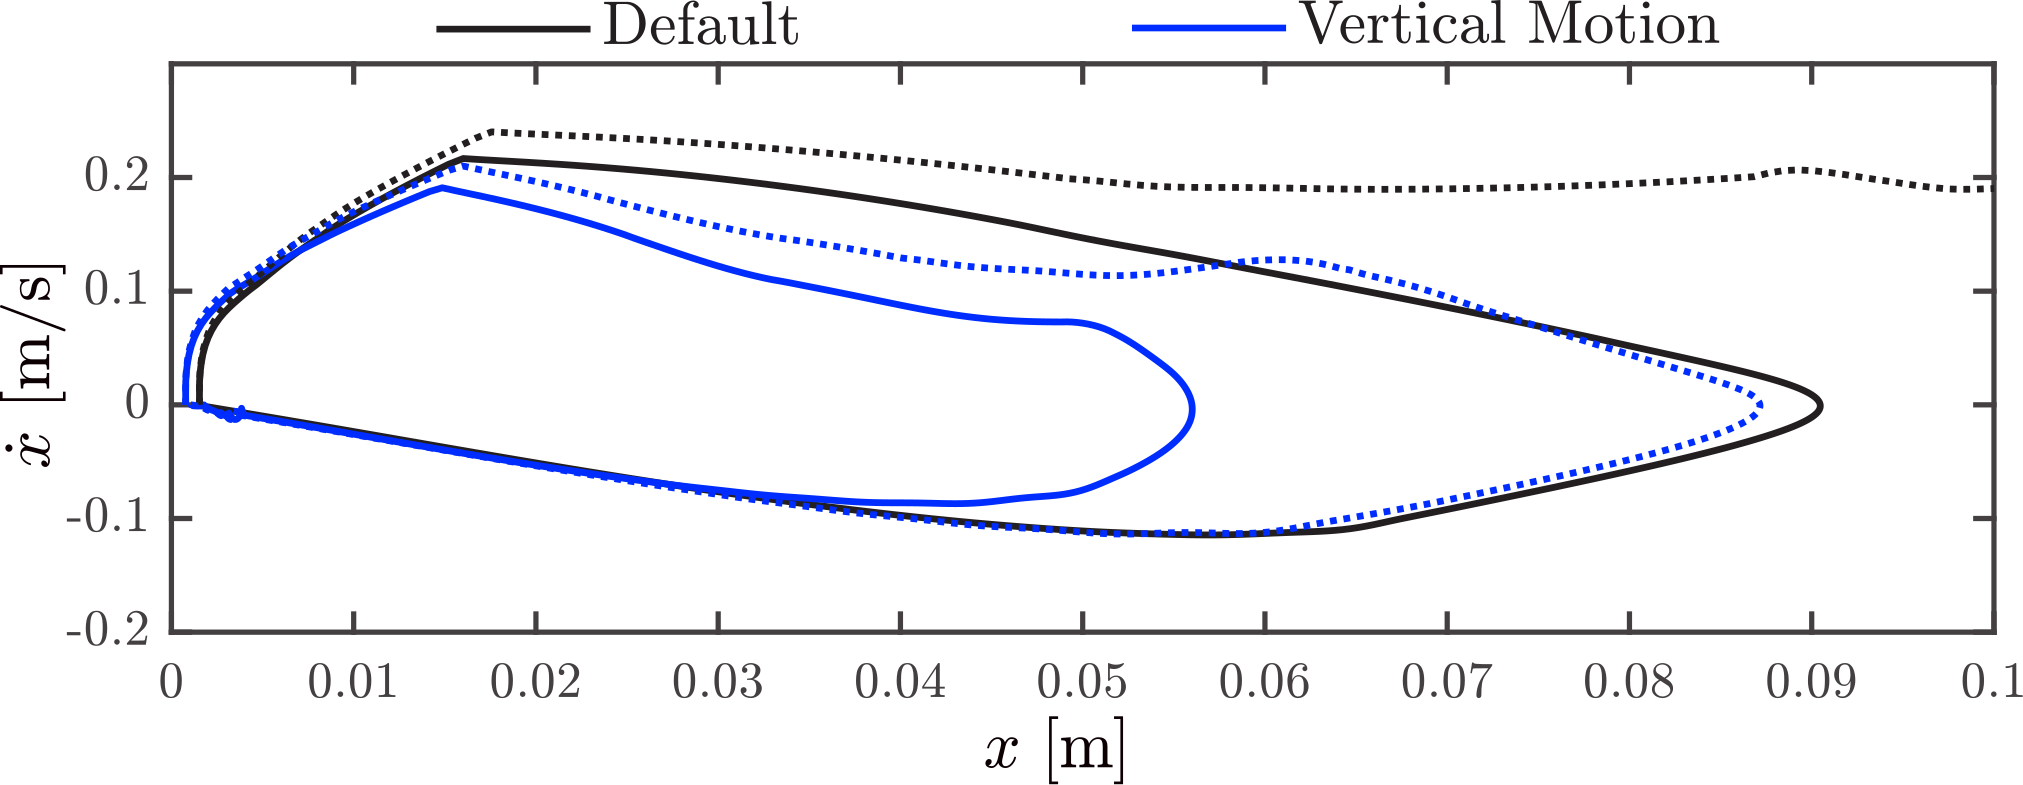
\includegraphics[width=0.9\textwidth]{STYLESTUFF/valcomparephase.png}
\caption{Phase plot of horitzontal \ac{CoM} motion in the sagittal plane for a push of $i=0.271$ [m/s] (solid) and a push of $i=0.295$ [m/s] (dotted).}
\label{fig:valcomparephase}
\end{figure}

In \figref{fig:valcomparetime}, time response plots are shown for a push of $i=0.271$ [m/s]. `Achieved' is the value after the \ac{QP} found a solution. For the vertical linear momentum rate $\dot{\mathbf{l}}_z$, the achieved tracks the desired fairly well. There is a larger difference between the desired and achieved horizontal linear momentum rate $\dot{\mathbf{l}}_x$ for both control setups. If the achieved is compared between the two setups, the vertical motion controller achieves almost double the amount $\dot{\mathbf{l}}_x$ the default control setup achieves from $0.1$ [s] until $0.25$ [s]. There is a small difference in achieved angular momentum rate observable. However, if there is looked at the pelvis error $\theta_{pel,y}$ and the torso error $\theta_{torso,y}$ in the fifth and sixth row, the vertical motion controller has a little less rotation error than the default setup, which shows no additional use of angular momentum strategies.
\begin{figure}
\centering
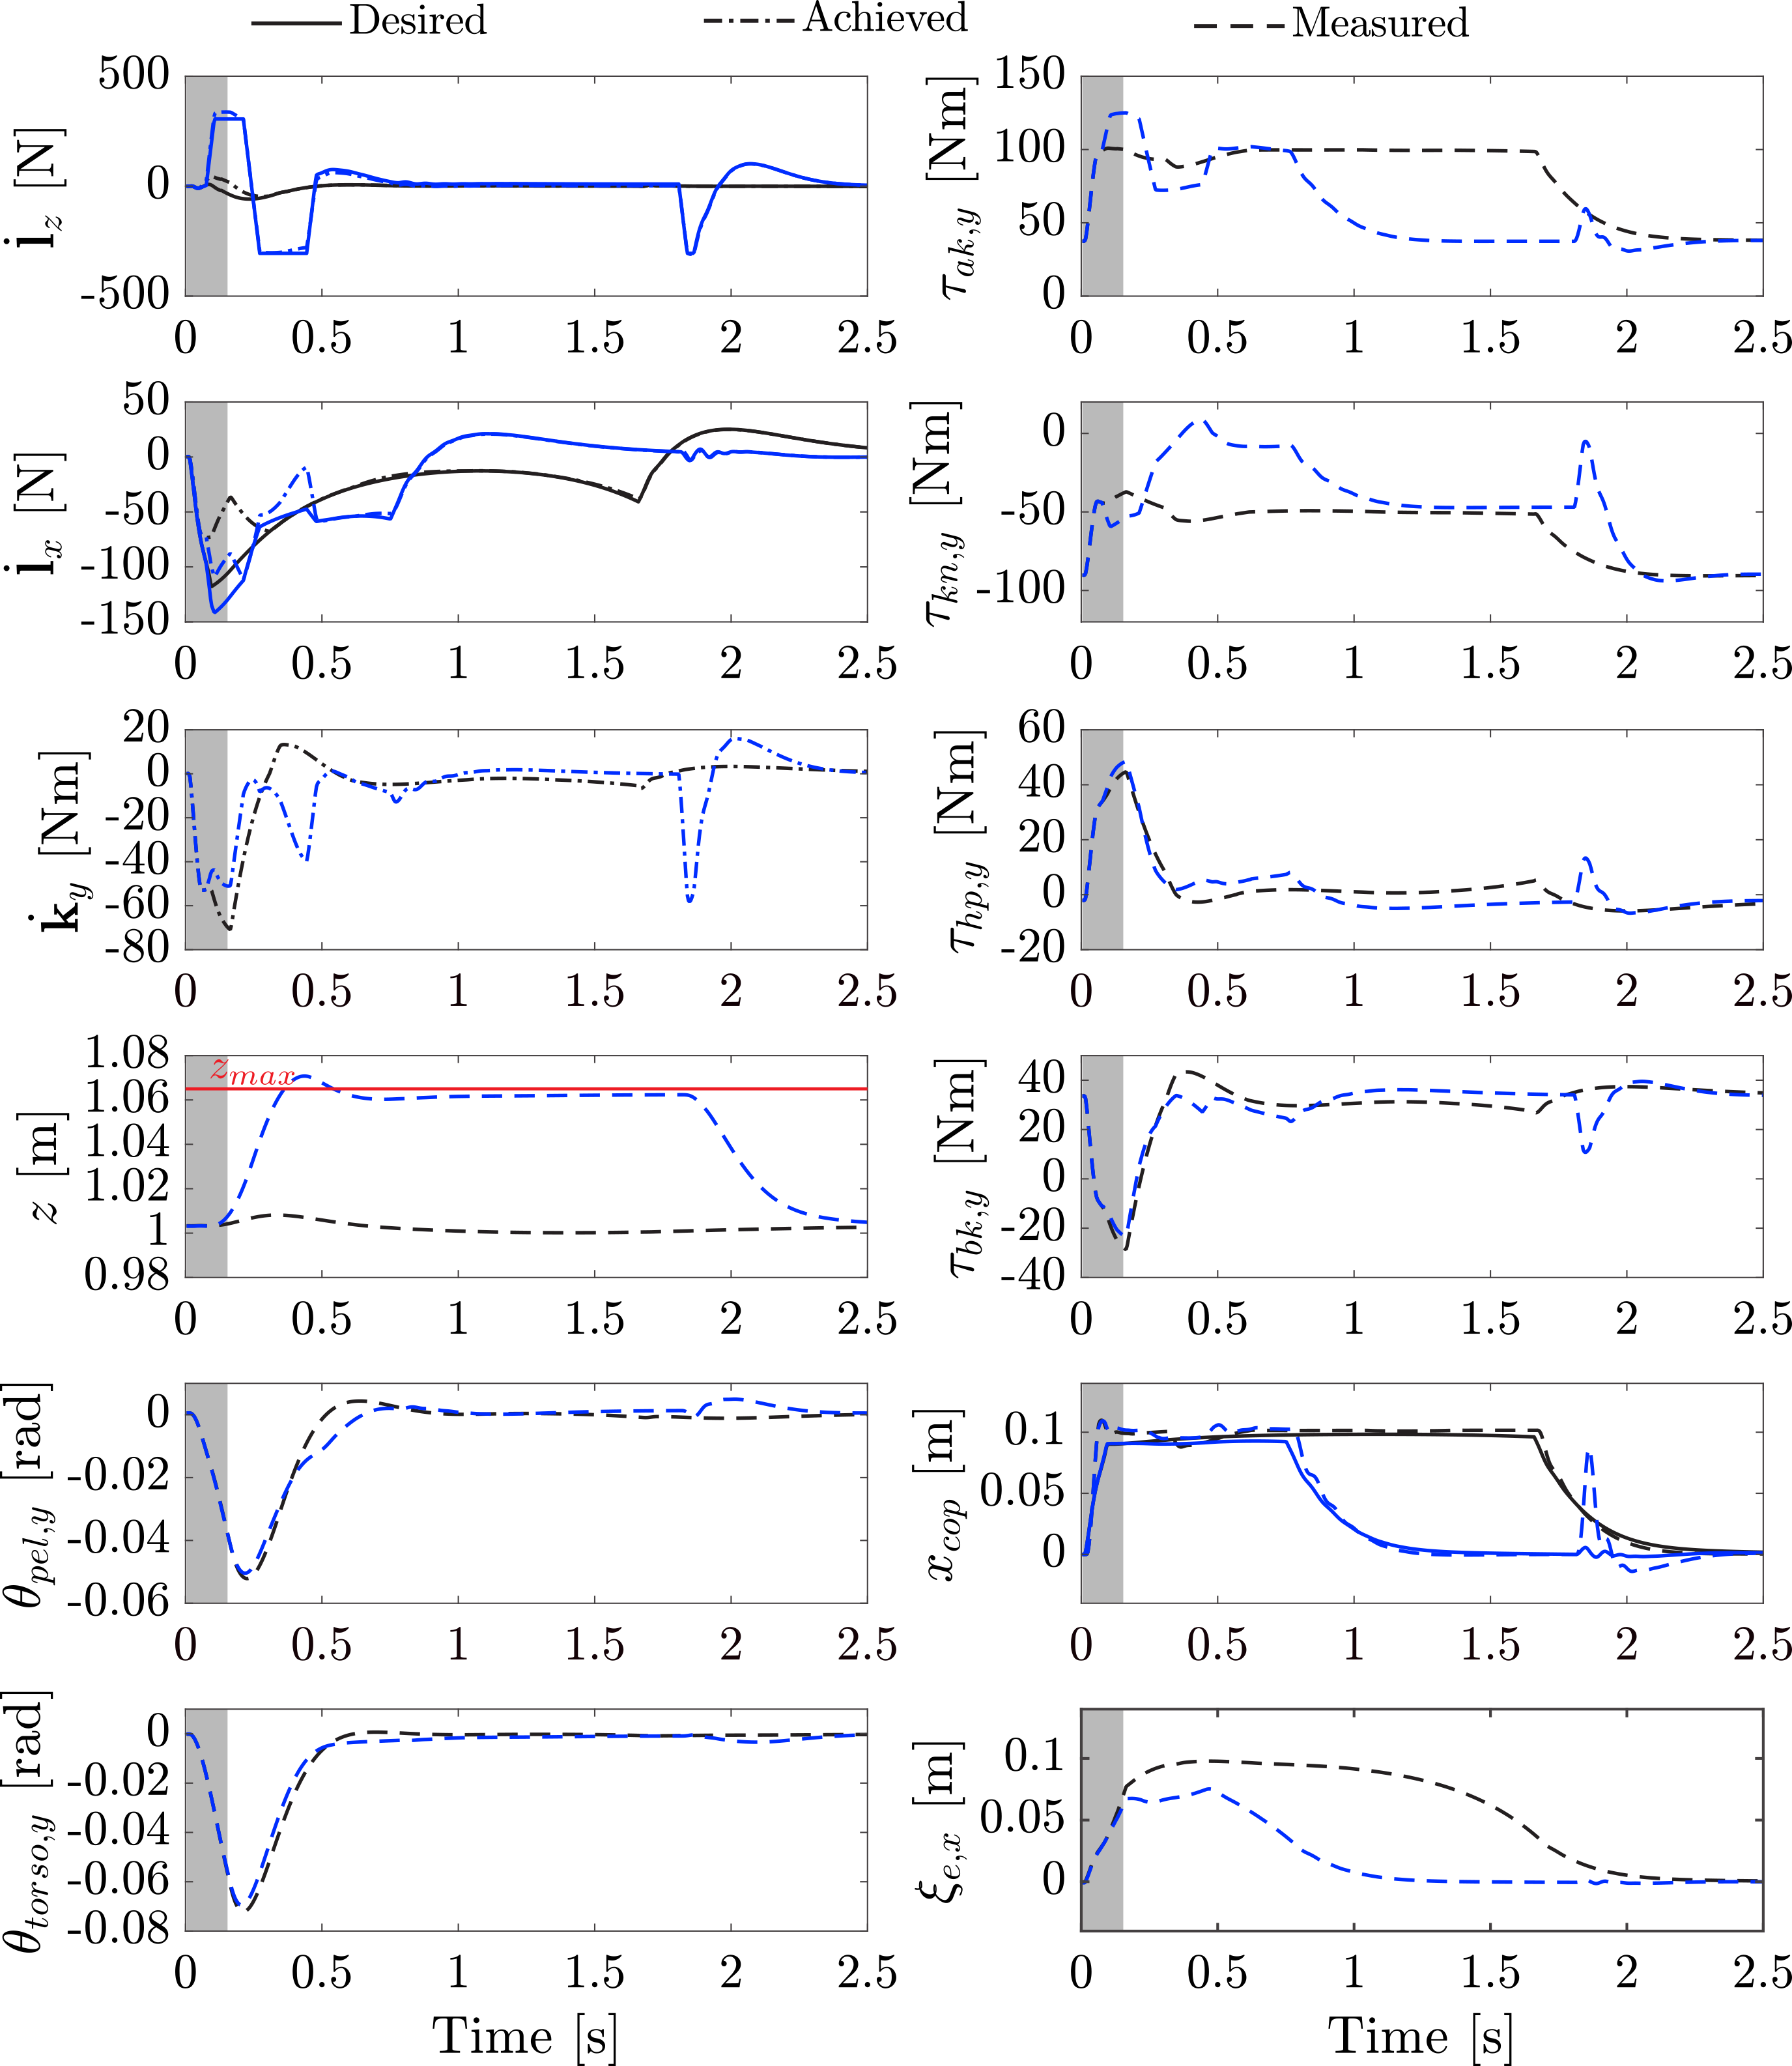
\includegraphics[width=1.0\textwidth]{STYLESTUFF/valcomparetime.png}
\caption{Time response plots for a push of $i=0.271$ [m/s] for the default setup (black) and the vertical motion controller (blue). `Achieved' is the value of the variable after the \ac{QP} found a solution. The gray area is where the push is applied.}
\label{fig:valcomparetime}
\end{figure}

In the right column of the figure, from the ankle torque $\tau_{ak,y}$, knee torque ankle torque $\tau_{kn,y}$, hip torque $\tau_{hp,y}$ and back torque $\tau_{bk,y}$, the difference in ankle and knee torque between both setups is the most noteworthy. The ankle torque has a higher peak for the vertical motion controller. Also, the ankle torque returns to the steady state value earlier than the default control setup. Similarly, the desired and measured \ac{CoP} returns to the steady state value earlier. This may be an indication of an increase in robustness for the push, as is observed in the phase plot as well. The knee torque is on average lower for the vertical motion controller. On average, the \ac{ICP} error $\xi_{e,x}$ is smaller, as expected.

\subsection{Valkyrie Hardware} 
Hardware tests on Valkyrie are conducted by applying a push in the back at chest height on the physical robot. An iLoad Pro Digital load censor \cite{iload} is used to measure the impulse of the push. The load sensor is mounted to an aluminum stick. On the other side of the load cell, a steel plate with a rubber surface is mounted. This prevents the robot from being damaged, and makes the push force data less dependent on contact impacts. In \figref{fig:pushhead}, the end of the push stick with the load sensor is depicted. In \figref{fig:authorpush}, the test setup is shown. A value of $\alpha_{\hat{\ddot{z}}_{c}}=0.8$ is used for the prediction of the vertical dynamics. The rest of the parameters are set to the same values as used in simulation.
\begin{figure}
\centering
  \begin{subfigure}{0.495\textwidth}
  \centering
  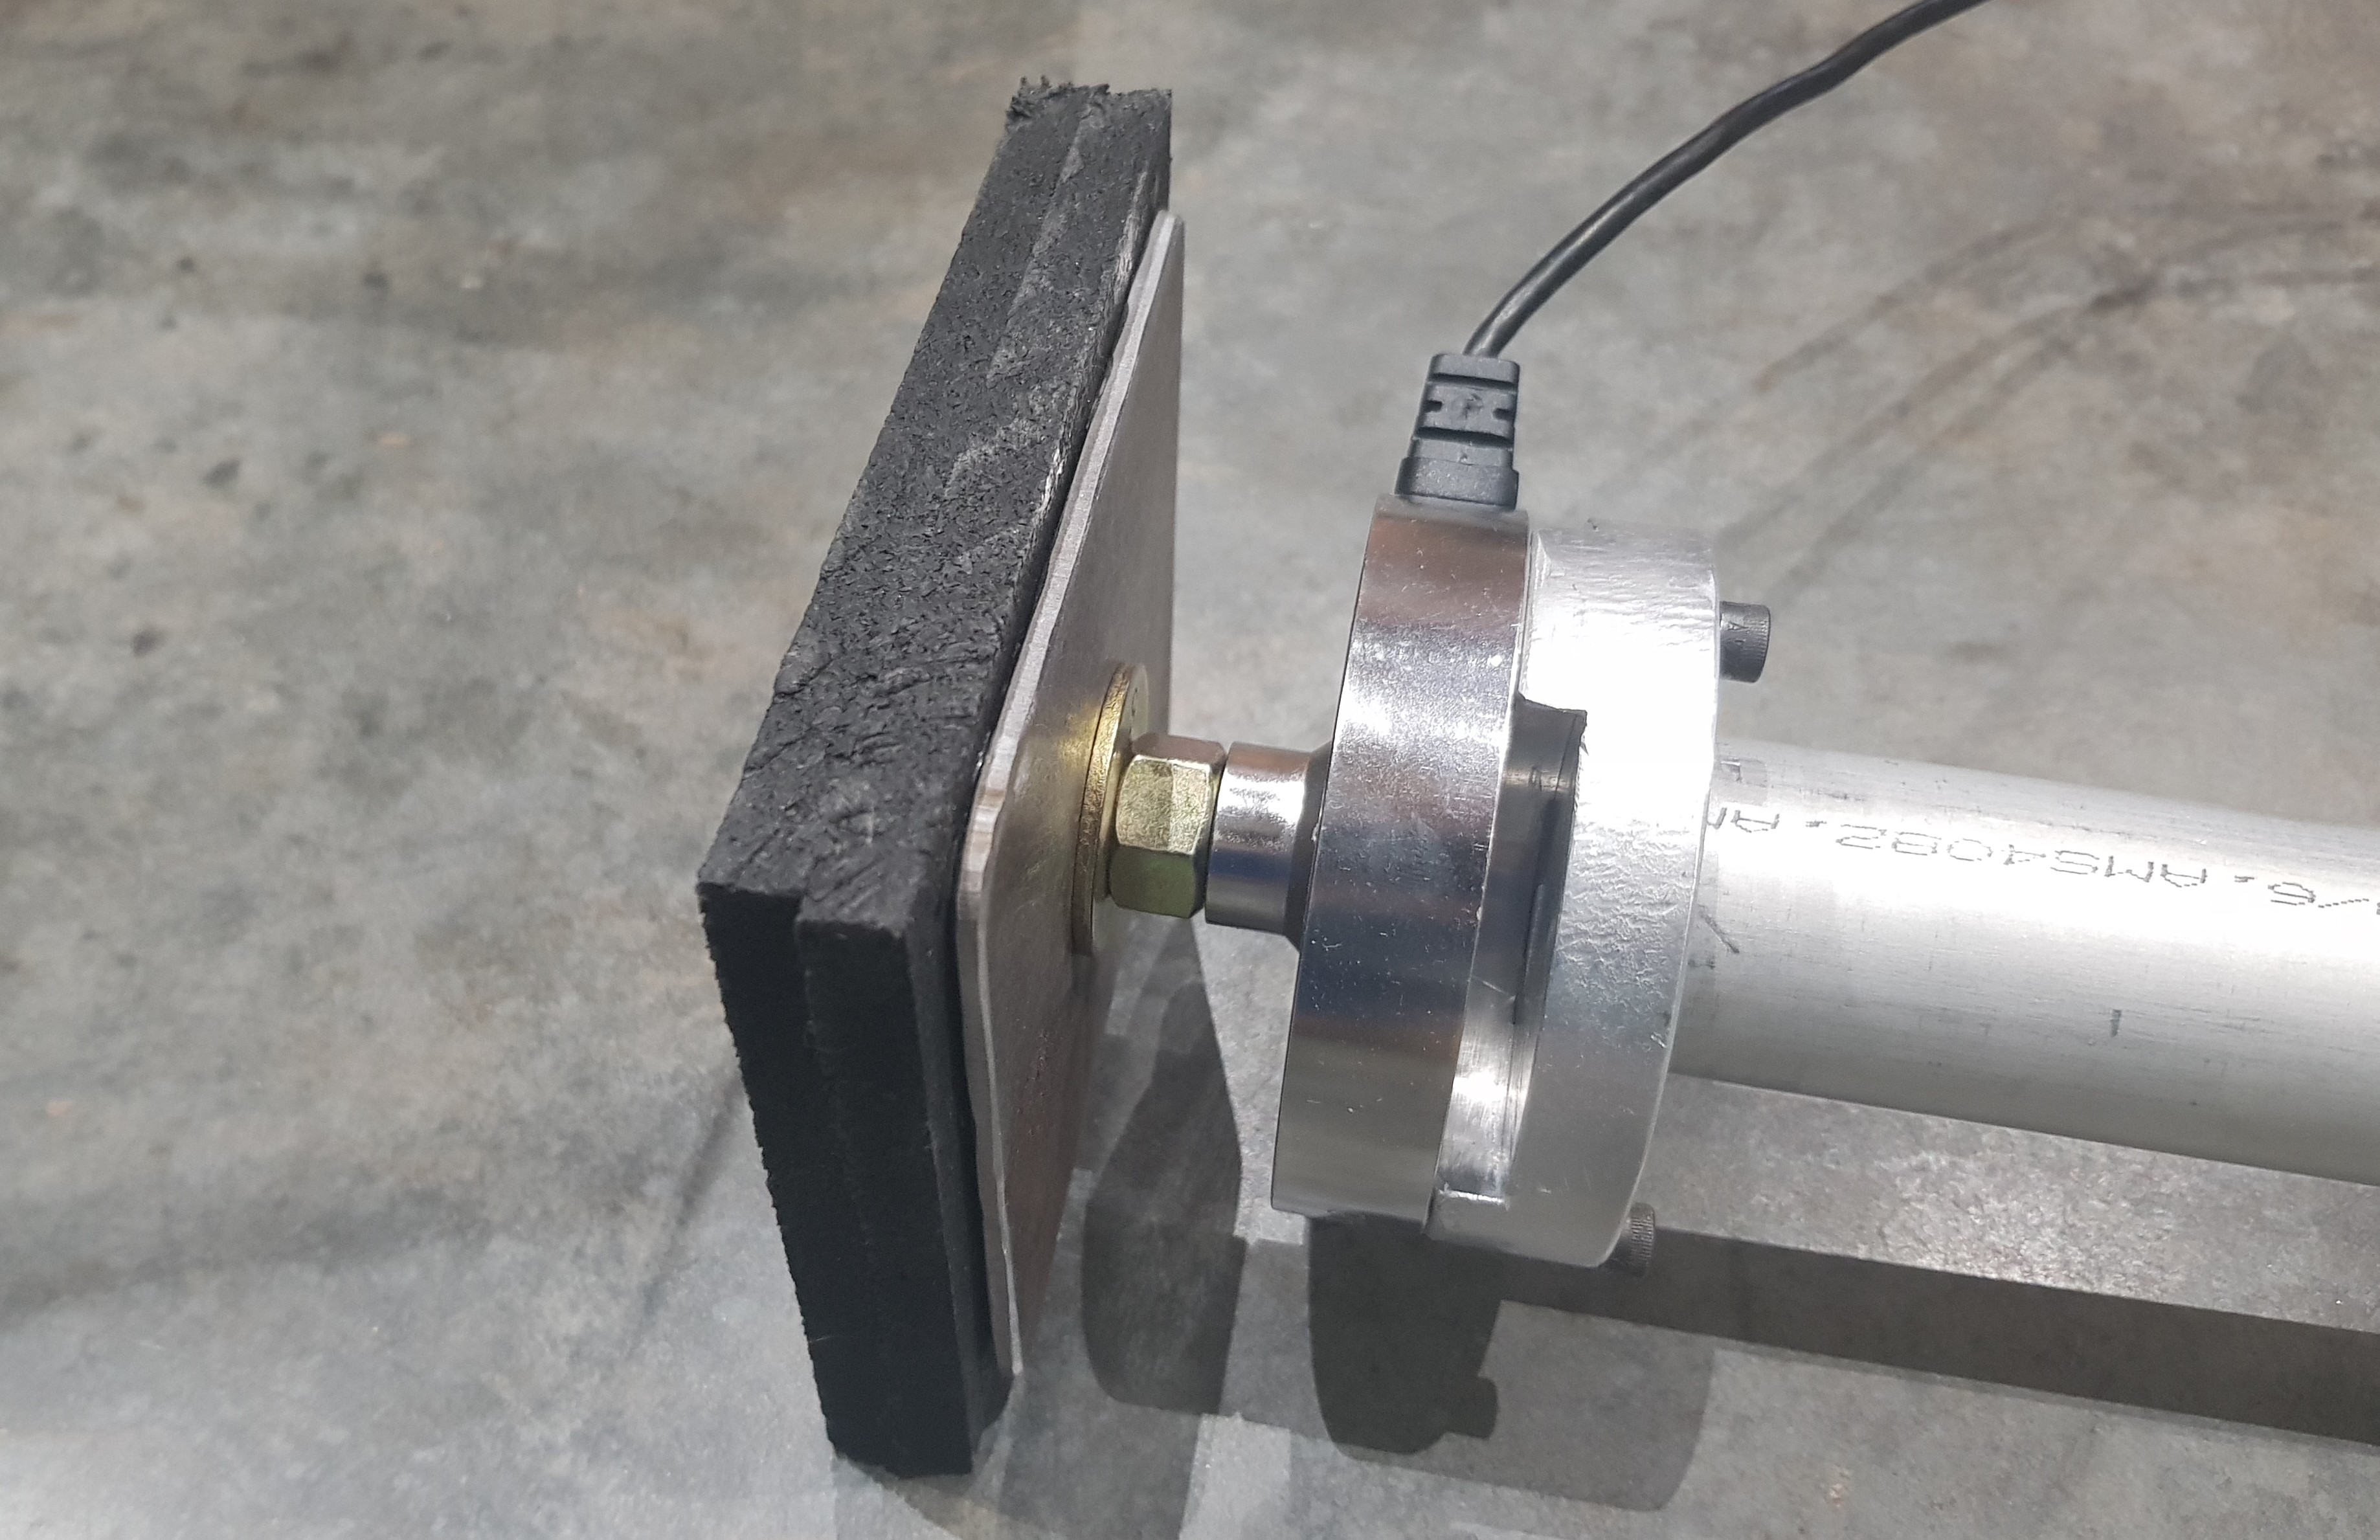
\includegraphics[width=.94\linewidth]{STYLESTUFF/pushhead.png}
   \caption{}
    \label{fig:pushhead}
  \end{subfigure}
  \begin{subfigure}{0.495\textwidth}
    \centering
  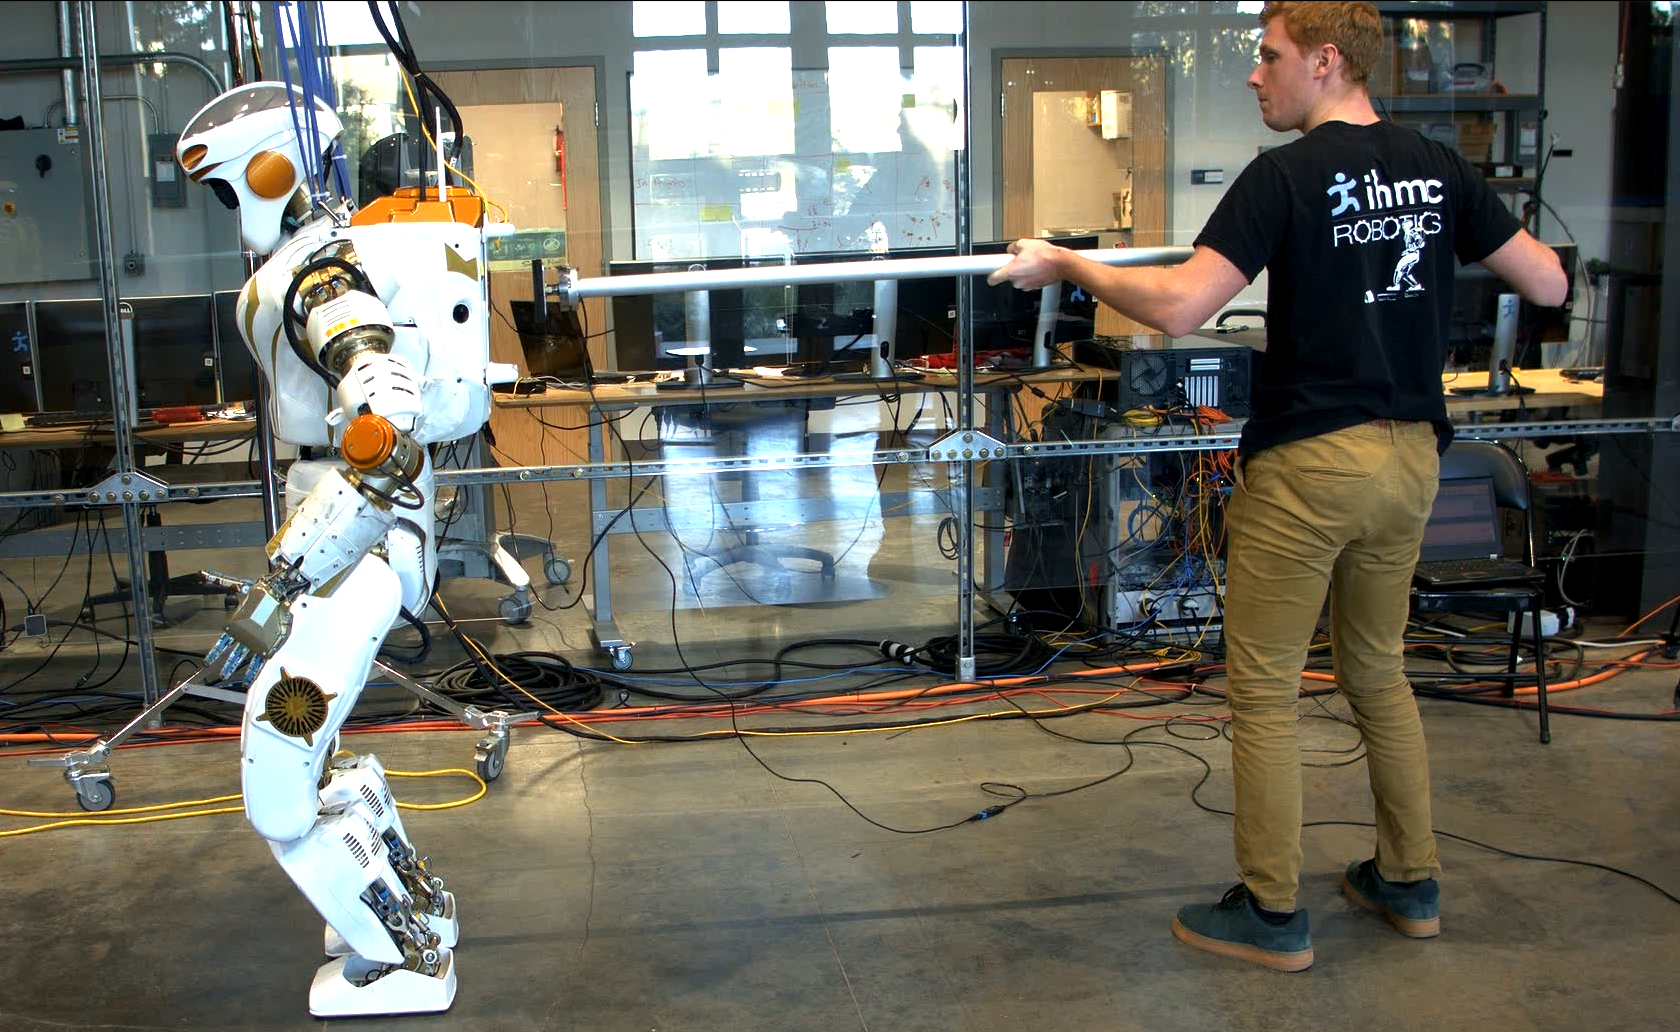
\includegraphics[width=.94\linewidth]{STYLESTUFF/authorpush.png}
  \caption{}
   \label{fig:authorpush}
  \end{subfigure}
  \caption{(a) Push head of push stick with the rubber surface, steel plate, load sensor and aluminum stick. (b) Tests setup, where the author applies a push using the push stick on Valkyrie.}
  \label{fig:pushsetup}
\end{figure}

\subsubsection{Maximum Recoverable Push}
To find the maximum recoverable push on hardware, a dozen test results are averaged where the \ac{CoM} of the robot came closer than $5$ [mm] from the polygon edge, but the robot still recovered. In \figref{fig:imp1}, the average force profile with the standard deviation of the $12$ pushes is depicted for the default setup. The average impulse is $35.3$ [Ns], which equals a normalized impulse of $i=\frac{35.3}{127.3}=0.277$ [m/s]. This is a slightly higher value than the impulse recoverable in simulation. In \figref{fig:imp2}, the average force profile with the standard deviation is depicted for the vertical motion controller. The average impulse is $37.6$ [Ns], which equals $i=0.295$ [m/s], which is an increase in recoverable push of approximately $7$\% compared to the default setup.
\begin{figure}
\centering
  \begin{subfigure}{0.32\textwidth}
  \centering
  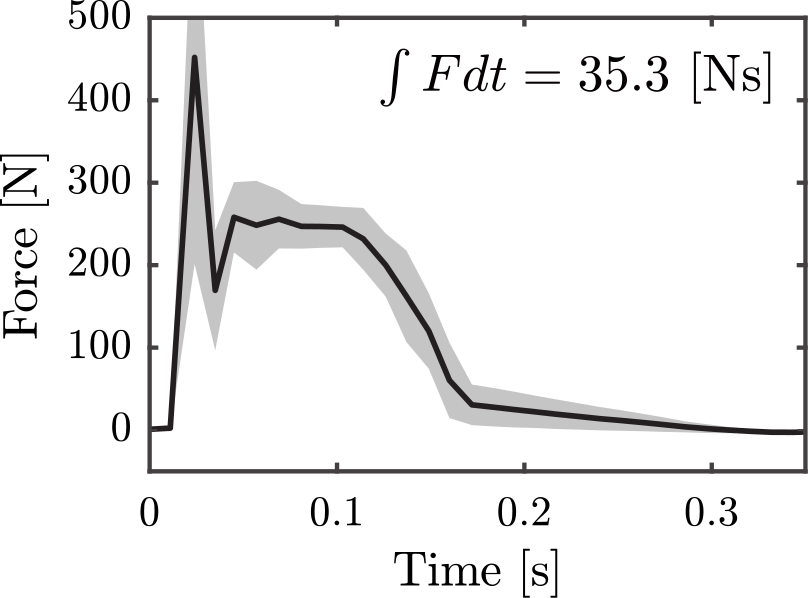
\includegraphics[width=.95\linewidth]{STYLESTUFF/impulsecompare1.png}
   \caption{}
    \label{fig:imp1}
  \end{subfigure}
    \begin{subfigure}{0.32\textwidth}
  \centering
  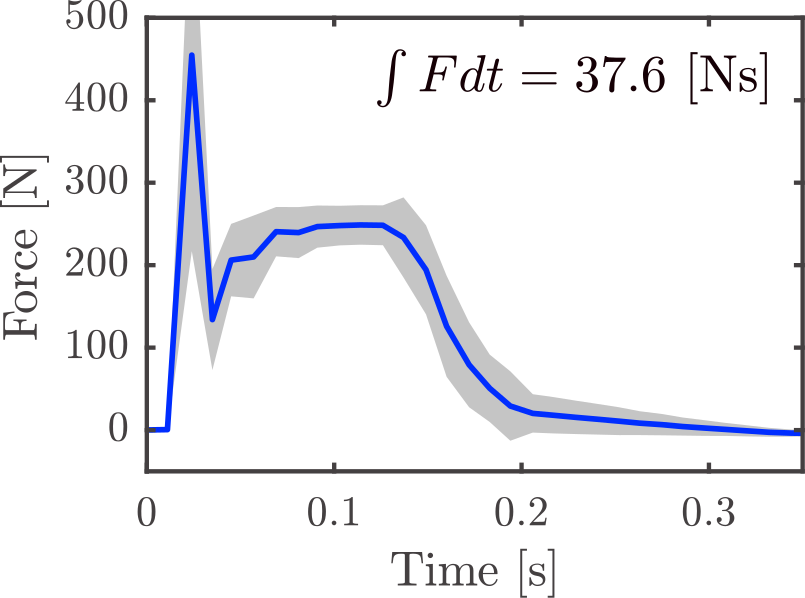
\includegraphics[width=.95\linewidth]{STYLESTUFF/impulsecompare2.png}
   \caption{}
    \label{fig:imp2}
  \end{subfigure}
  \begin{subfigure}{0.32\textwidth}
    \centering
  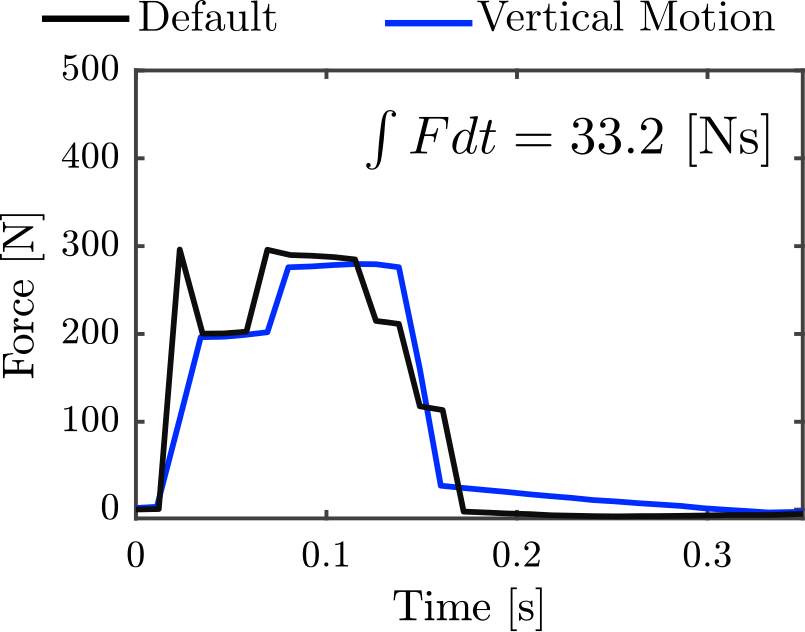
\includegraphics[width=.95\linewidth]{STYLESTUFF/impulsecompare31.png}
  \caption{}
   \label{fig:imp3}
  \end{subfigure}
  \caption{Average impulse of $12$ pushes, where the \ac{CoM} came closer than $5$ [mm] from the polygon edge for the (a) default setup and (b) vertical motion controller. (c) Two picks of pushes, where the force profile and integrated force applied on both setups were similar. }
  \label{fig:impulsecompare}
\end{figure}

\begin{figure}
\centering
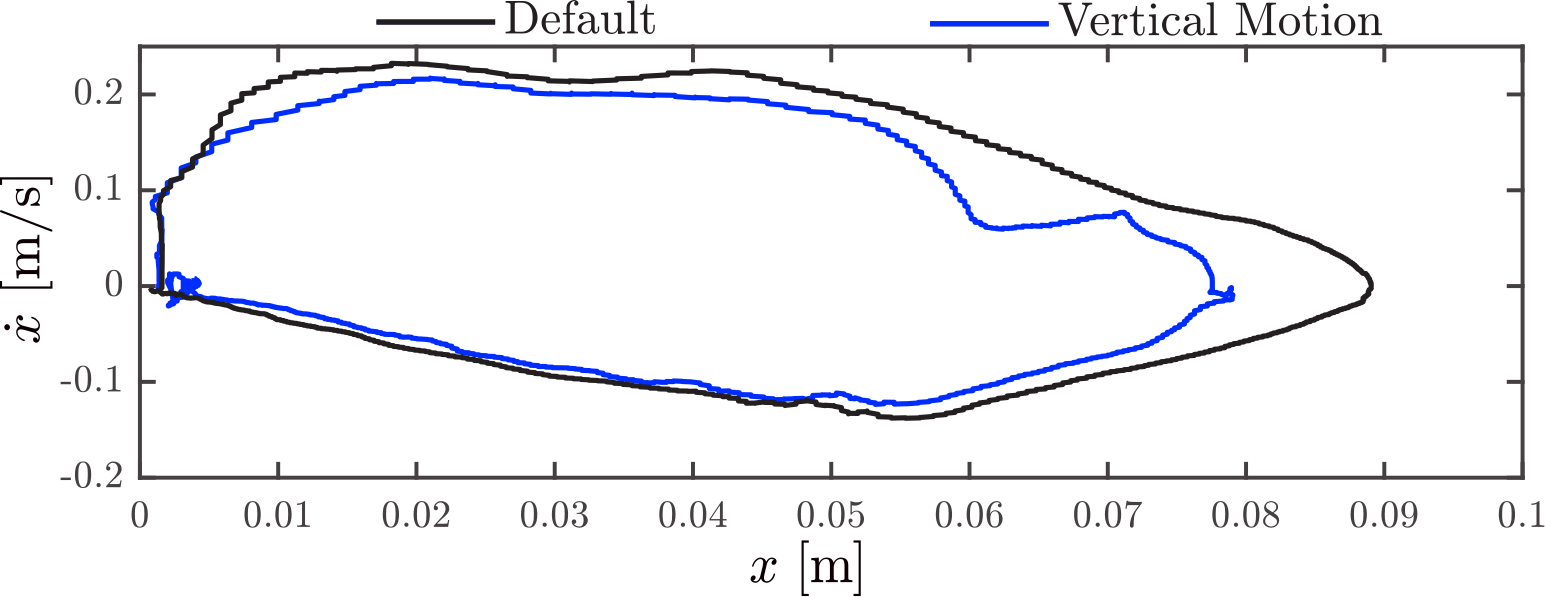
\includegraphics[width=0.7\textwidth]{STYLESTUFF/valcomparephaseHW.png}
\caption{Phase plot of forward \ac{CoM} motion for a push of $i=0.261$ [m/s].}
\label{fig:valcomparephaseHW}
\end{figure}
\begin{figure}
\centering
  \begin{tabular}{ccccccc}
    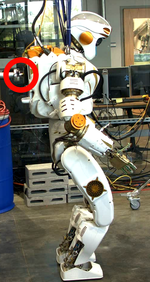
\includegraphics[width=0.7in]{STYLESTUFF/val1zr_C} &
    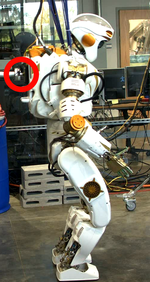
\includegraphics[width=0.7in]{STYLESTUFF/val2zr_30} &
    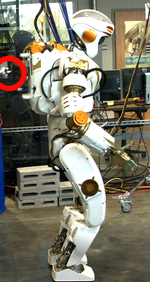
\includegraphics[width=0.7in]{STYLESTUFF/val3zr_30} &
    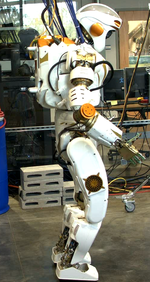
\includegraphics[width=0.7in]{STYLESTUFF/val4z_30} &
    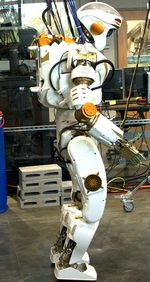
\includegraphics[width=0.7in]{STYLESTUFF/val5z_30} &
    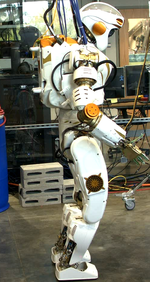
\includegraphics[width=0.7in]{STYLESTUFF/val6z_30} &
    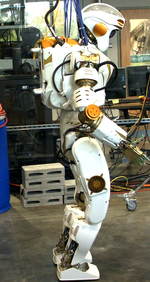
\includegraphics[width=0.7in]{STYLESTUFF/val7z_30} ~\\[2ex]
     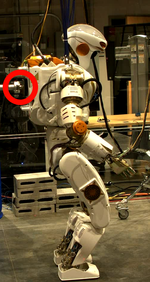
\includegraphics[width=0.7in]{STYLESTUFF/val1dr_C} &
    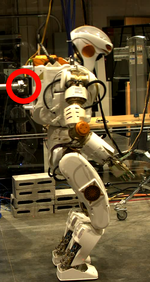
\includegraphics[width=0.7in]{STYLESTUFF/val2dr_30} &
    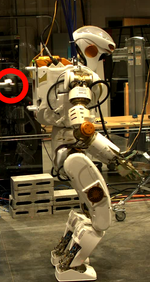
\includegraphics[width=0.7in]{STYLESTUFF/val3dr_30} &
    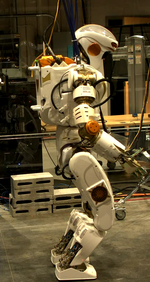
\includegraphics[width=0.7in]{STYLESTUFF/val4d_30} &
    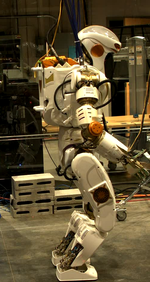
\includegraphics[width=0.7in]{STYLESTUFF/val5d_30} &
    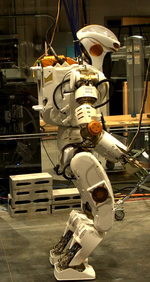
\includegraphics[width=0.7in]{STYLESTUFF/val6d_30} &
    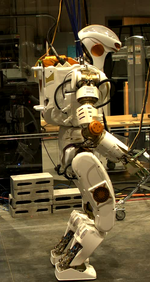
\includegraphics[width=0.7in]{STYLESTUFF/val7d_30} \\
    $a$&
    $b$&
    $c$&
    $d$&
    $e$&
    $f$&
    $g$\\
  \end{tabular}
  \caption{Time-lapse of Valkyrie recovering from a push using vertical motion (top row) and using the default controller setup (bottom row). The letters below the columns match with the letters next to the yellow lines in Figure \ref{fig:valcomparetimeHW}. The push rod tip is encircled in red.}
  \label{fig:val}
\end{figure}

\subsubsection{Comparison of Equal Push} 
By selecting a force profile from each setup where the integrated force is approximately equal and the force profiles have a comparable shape, a comparison can be made between both control setups under a similar disturbance. In \figref{fig:imp3}, the two compared force profiles are shown. Both profiles have an impulse of $33.2$ [Ns], which is equal to $i=0.261$ [m/s]. In \figref{fig:valcomparephaseHW}, a phase plot for the sagittal horizontal motion is depicted. Like in simulation, the vertical motion covers a smaller area. 

In \figref{fig:val}, a time-lapse is shown for both control setups after these pushes. The letters under each column match with the letters next to the vertical yellow lines in \figref{fig:valcomparetimeHW}. In \figref{fig:valcomparetimeHW}, time response plots are shown for the pushes of $i=0.261$ [m/s]. Note how the vertical lines leave the gray area, when in the \figref{fig:val} the red encircled push head loses contact with the robot. 
\begin{figure}
\centering
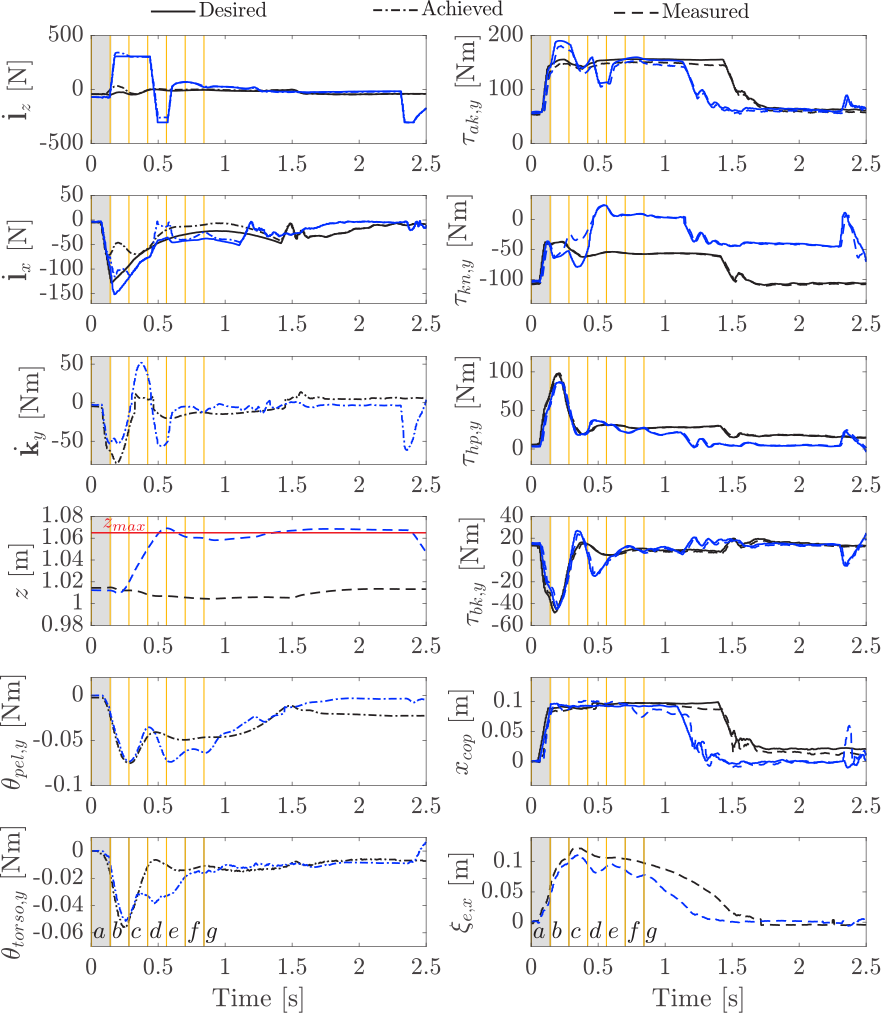
\includegraphics[width=1.0\textwidth]{STYLESTUFF/valcomparetimeHW.png}
\caption{Time response plots for a push of $i=0.261$ [m/s] for the default setup (black) and the vertical motion controller (blue). All joint torques, except for the back, are the average over left and right.}
\label{fig:valcomparetimeHW}
\end{figure}

Also note how the timing of each `bang', visible in the vertical linear momentum rate $\dot{\mathbf{l}}_z$, is different compared to the results observed in simulation. This might be a reason why a larger value of $\alpha_{\hat{\ddot{z}}_{c}}$ could be used. The $\dot{\mathbf{l}}_x$ plots are comparable with the simulation results. The achieved angular momentum rate $\dot{\mathbf{k}}_y$ of the vertical motion controller has a relatively larger overshoot than in simulation. However, the resulting pelvis and torso rotation errors are not larger for the vertical motion controller compared to the default setup, which shows no additional use of angular momentum strategies, like in simulation. 

In the right column of the figure, the torques have a desired and a measured value, as the torques of the robot are PD controlled with electrical current as input. Like in simulation, the differences in ankle torque and knee torque between the default setup and the vertical motion controller are the most noteworthy. For the vertical motion controller, the ankle torque has a higher peak, but returns quicker to steady-state, like in simulation.  The \ac{CoP} also returns earlier to steady state, which shows a slight increase in robustness for the applied push. Equivalently, the average \ac{ICP} error is again smaller for the vertical motion controller.

\subsection{Atlas Hardware}
Next to the Valkyrie tests, tests are conducted on Boston Dynamics' Atlas humanoid robot. An alternative experimental setup is used to test push recovery on hardware. A medicine ball with mass $m_{ball}=13.6$ [kg] is hung from the ceiling at the robotics lab of \ac{IHMC}. To push the robot, the ball can be released from a certain distance. The impulse on the robot is assumed to be only depending on the difference in potential energy of the ball between release and its lowest position. To protect the robot from the impact of the ball, a wooden plate is mounted on the frame of the robot. In \figref{fig:atlassetup}, the test setup is depicted. The length $\lball$ from the horizontal release location to the dead point of the pendulum is used to calculate the impulse applied on the robot. To release the ball, a simple mechanism is made in an attempt to get a more constant initial ball position. This mechanism is depicted in \figref{fig:ballrelease}. By pulling the aluminum pin, the loop on the rope will slide off the pin.
\begin{figure}
\centering
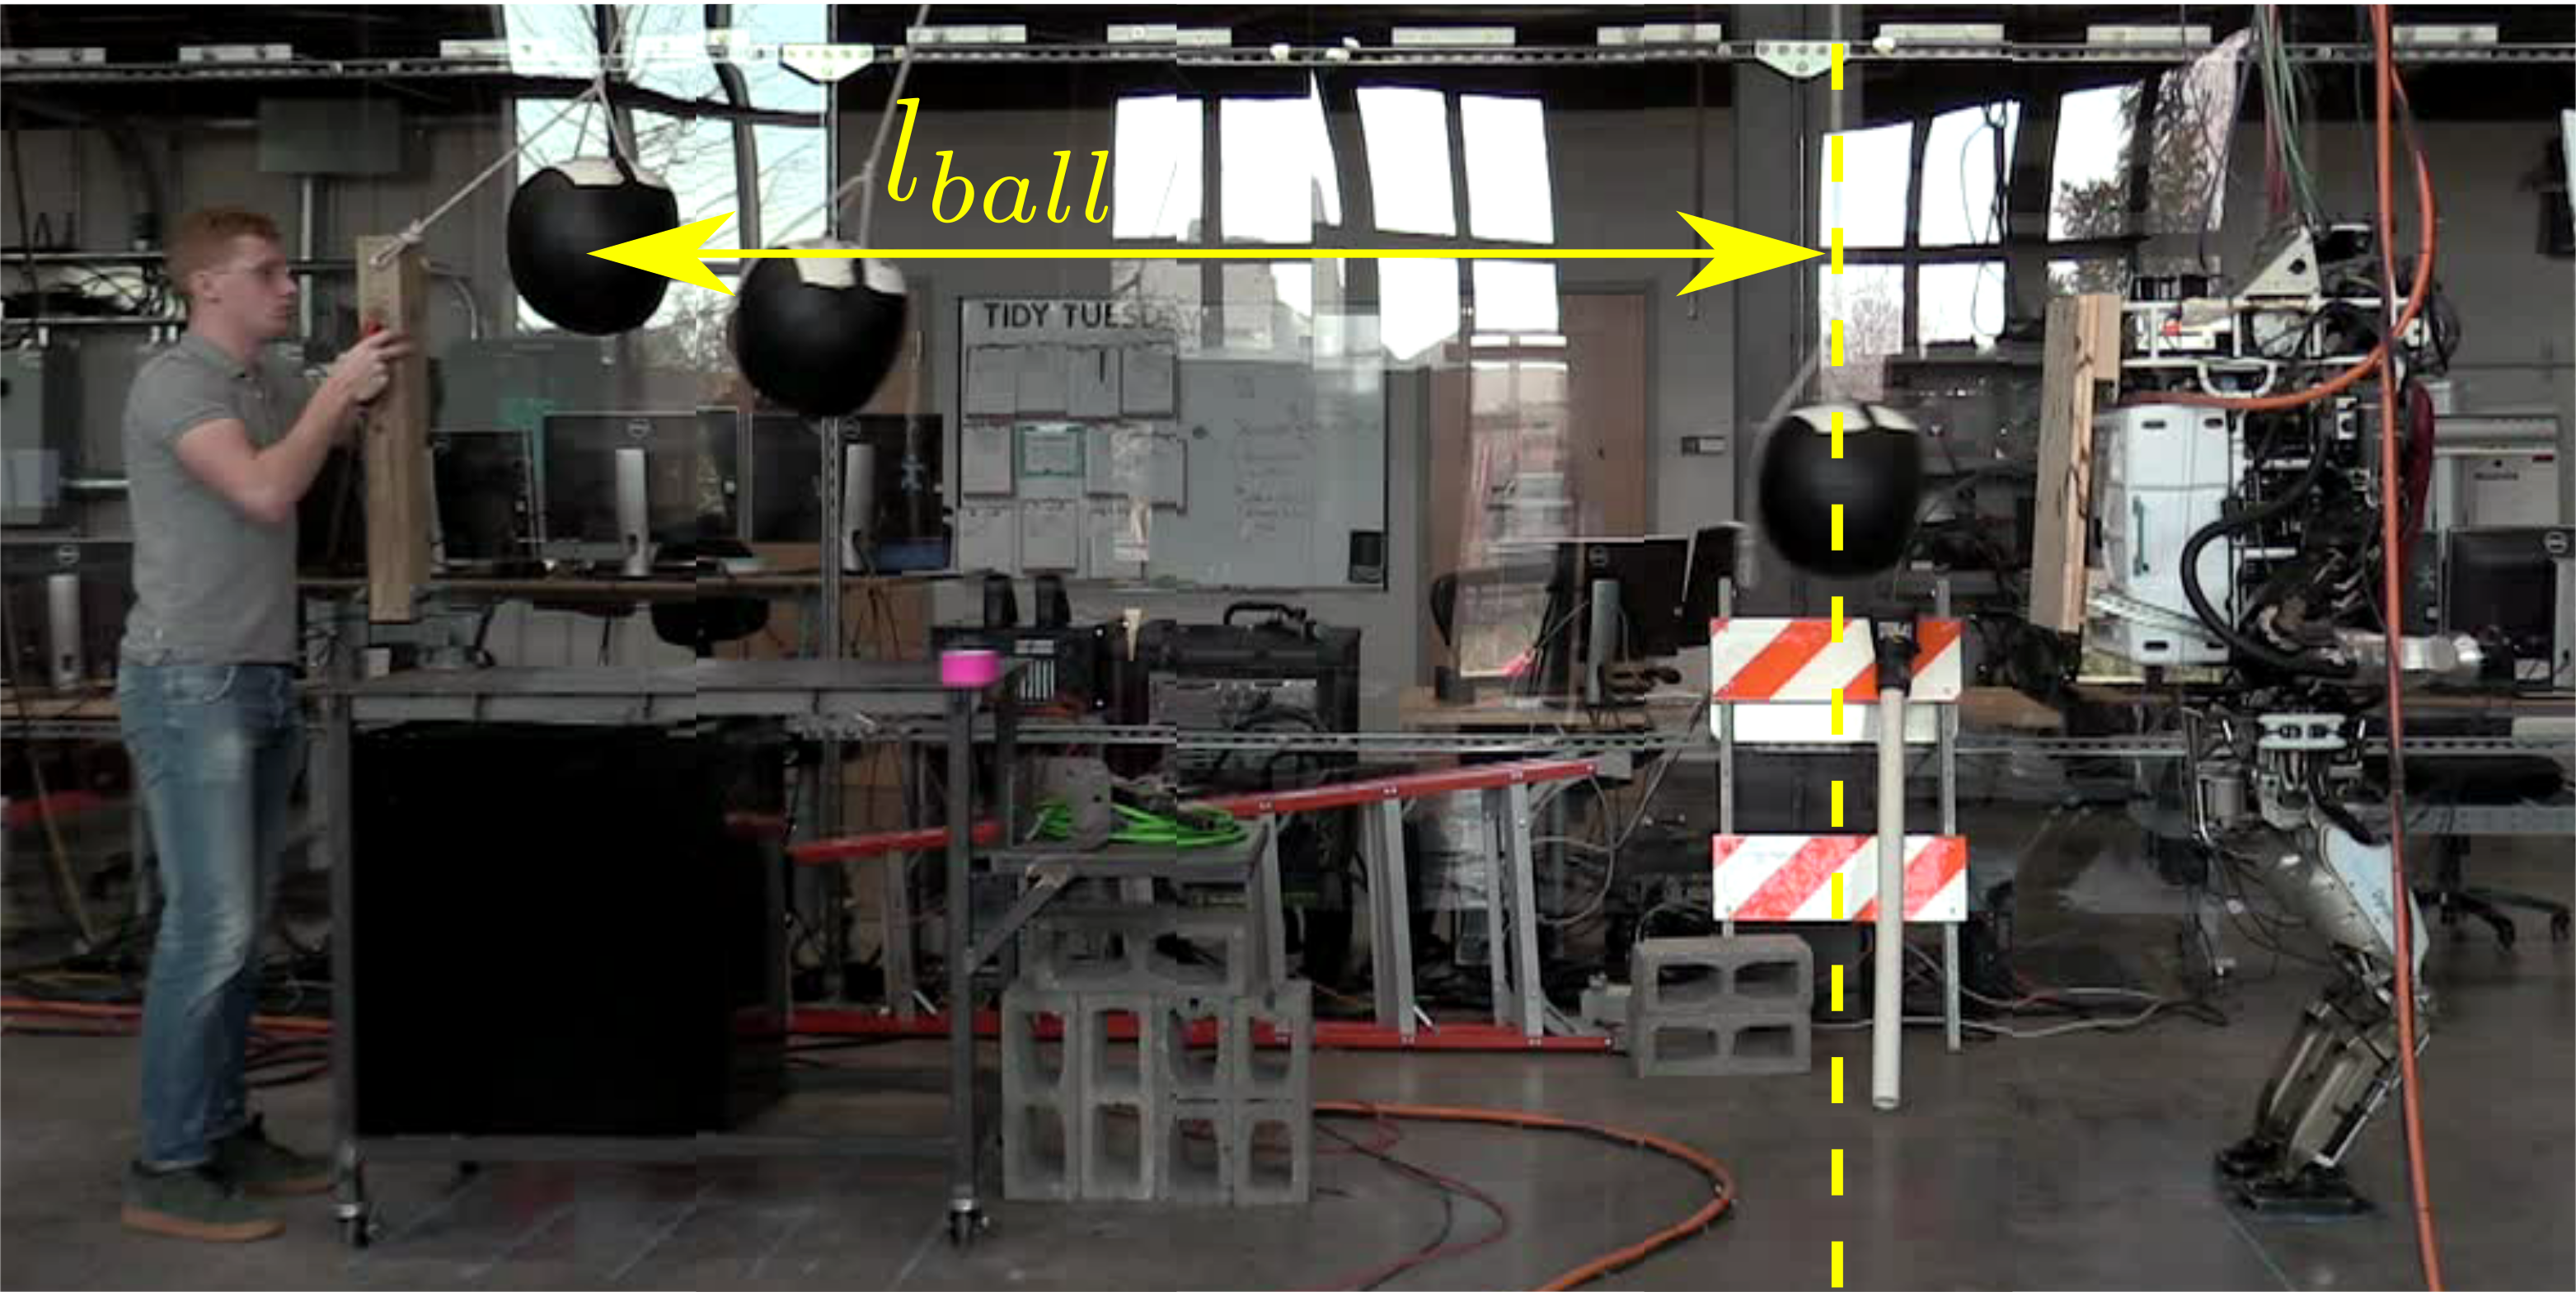
\includegraphics[width=0.99\textwidth]{STYLESTUFF/atlassetup.png}
\caption{Experimental setup for hardware tests on Atlas.}
\label{fig:atlassetup}
\end{figure}
\begin{figure}
\centering
\includegraphics[width=0.7\textwidth]{STYLESTUFF/ballrelease.png}
\caption{Release mechanism for the medicine ball tests.}
\label{fig:ballrelease}
\end{figure}

\subsubsection{Maximum Recoverable Push}
A total of $50$ experiments are conducted, but no clear improvement in recovery compared to the default controller could be observed. Different initial heights for the robot are tried, by gradually lowering the default initial height of $z_0=1.12$ [m] down to $z_0=1.05$ [m]. Lowering the initial height made the relative increase in recoverable push compared to the default setup larger in simulation, but recovery on hardware did not improve. The increase in recoverable push compared to the default controller for these initial heights in simulation are in the range $6-10$\%. In another attempt to improve recovery, the foot polygon size for the whole-body \ac{QP} was enlarged as well. The robot would handle larger impulses, but the difference observed between the two control setups was still neglectable.

Additionally, in an attempt to improve recovery for the vertical motion controller, a gain for joint torque control is tuned. From the data collected from earlier tests, it was observed that the measured \ac{CoP} had a relatively large tracking error with $\rcopd$, especially during the second `bang' of the control law. The joint torques on Atlas are controlled using an input current $I$ and are computed as follows \cite{koolen2016design}:
\begin{align}
	I &= I_{\tau} + I_{\dot{q}},\\
	I_{\tau} &= k_{ff_{\tau}}\tau_{d} + k_{\tau}(\tau_{d} - \tau),\\
	I_{\dot{q}} &= k_{ff_{\dot{q}}}\dot{q} + k_{\dot{q}}\bigg(\int \ddot{q}_d dt - \dot{q} \bigg),
\end{align}
where $k_{ff_{\tau}}$ and $k_{\tau}$ are a feedforward and feedback gain on tracking of desired joint torques respectively. The gain $k_{ff_{\dot{q}}}$ is a feedforward gain to compensate the oil flow in the cylinder as the actuator is moving. The gain $k_{\dot{q}}$ is a feedback gain on desired joint velocity, where the desired joint velocity is computed by integration of the desired joint acceleration $\ddot{q}_d$, an output of the whole-body \ac{QP}. For the tests, \ac{CoP} tracking improved by increasing the gain $k_{\dot{q}}$ from $15.0$ to $40.0$. In \figref{fig:atlascop}, the difference in \ac{CoP} tracking between the two gain values is depicted during the two `bangs' of the control law. Note how tracking improved during the second `bang' after increasing the gain. Unfortunately, push recovery did not noticeably improve.

\begin{figure}
\centering
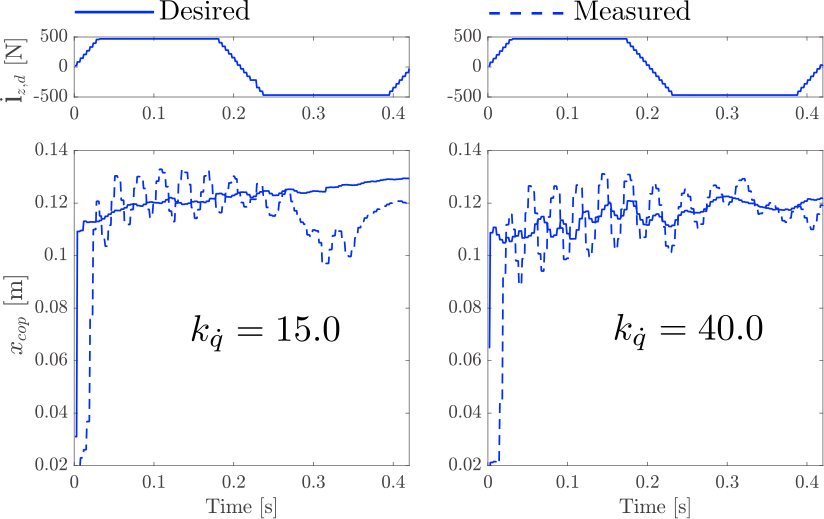
\includegraphics[width=0.9\textwidth]{STYLESTUFF/atlascop.png}
\caption{\ac{CoP} tracking during the two `bangs' of the vertical motion control law. In the left column, $k_{\dot{q}}=15.0$. In the right column, $k_{\dot{q}}=40.0$. For illustration of the `bangs', $\dotldz$ is graphed. }
\label{fig:atlascop}
\end{figure}

\subsubsection{Comparison of Equal Push}
For an initial height of $z_0=1.10$ [m], a maximum height of $\zmax=1.17$ [m] and a vertical acceleration of $\ddzc=[5.0]$ [m/s$^2$], a series of $20$ tests for each control setup are conducted to investigate the responses after an equal push. The increase in recoverable push for these parameters in simulation is approximately $8$\%, which shows that there is a noticable difference for the two control setups for this configuration. For the hardware tests, an initial ball position of $\lball=2.54$ [m] is used. The difference in ball height $\delta z_{ball}$ is computed as follows:
\begin{equation}
	\delta z_{ball} = l_{rope} - \sqrt{l_{rope}^2-l_{ball}^2} = 6.12-\sqrt{6.12^2 - 2.54^2} = 0.543 \quad \text{[m]},
\end{equation}
where $l_{rope}$ is the length of the rope between the ceiling attachment point and the ball. The impulse applied on the robot is calculated as:
\begin{equation}
m_{ball}\dot{x}_{ball} = m_{ball}\sqrt{2g\delta z_{ball} } = 13.6\sqrt{2 \cdot 9.81 \cdot 0.543} = 44.4 \quad \text{[Ns]},
\end{equation}
where $\dot{x}_{ball}$ is the velocity of the ball. Normalizing the impulse, like with the Valkyrie tests, results in a value of $i=\frac{44.4}{155.9}=0.285$ [m/s]. From the logging camera it is observed that the push duration is about $0.03-0.05$ [s].

In \figref{fig:atlasphaseHW}, phase plots are shown for these tests. The thin transparent lines show the responses after each individual test. The bold plots show the averages of all results. The average phase plot for the vertical motion controller covers a slightly smaller area. However, the individual responses have a wider distribution, which shows a less predictable behavior. The wider distribution was also visible on the robot, as sometimes the robot would visibly almost fall over, and sometimes recover relatively quick. A reason for this could be that the robot moves when using height variation, which might cause larger sensing and actuation errors. Also, for the vertical motion controller, there is a slight increase in velocity observable after approximately $x=0.06$ [m] in the upper half of the phase plot. Assuming no angular momentum change in the robot, an increase in velocity can be caused by the \ac{CoP} still tracking poorly. A reason for this could be that for the tests in the phase plot a vertical acceleration of $\ddzc=5.0$ [m/s$^2$] was used, instead of the $\ddzc=3.2$ [m/s$^2$] used in the tuning of the gain $k_{\dot{q}}$, where tracking of the \ac{CoP} was relatively better.

\begin{figure}
\centering
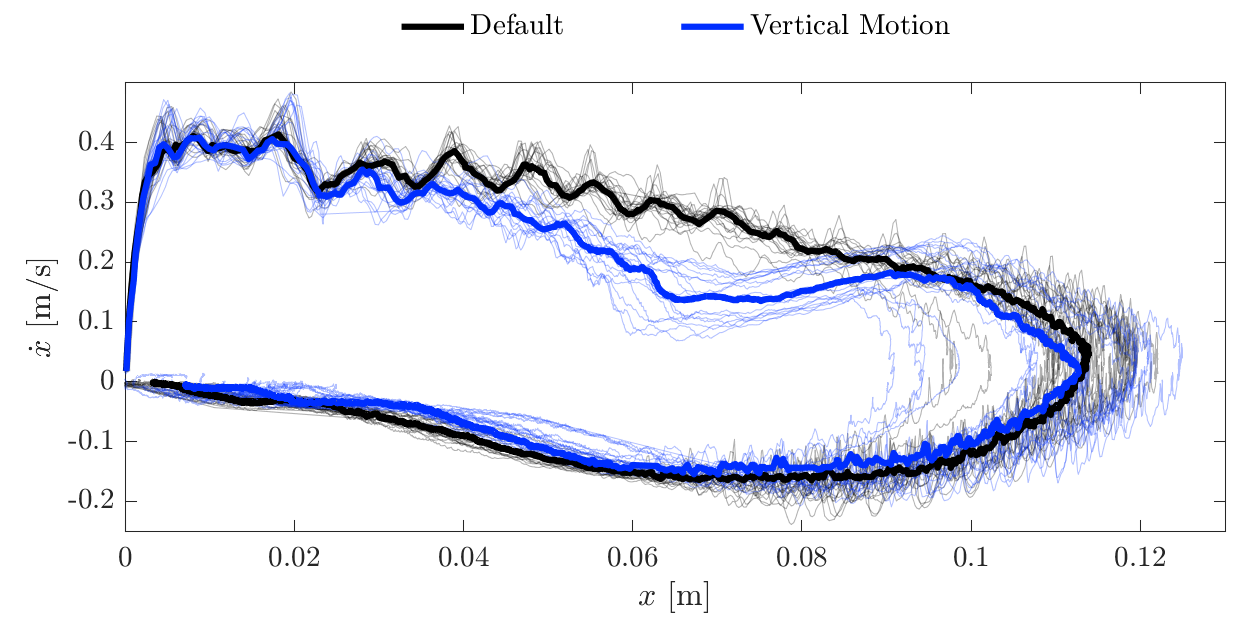
\includegraphics[width=0.9\textwidth]{STYLESTUFF/atlasphaseHW.png}
\caption{Phase plots of $20$ Atlas hardware tests for each setup (thin transparent) with the averaged data for each setup (bold).}
\label{fig:atlasphaseHW}
\end{figure}

\subsection{Comparison with Capture Regions}
If is assumed that the difference in recovery between the default setup and the vertical motion controller is equal to the difference between the LIP and the \ac{VHIP}, a comparison can be made between the push recovery tests and the \ac{VHIP} capture regions of Chapter \ref{chap:regions}.

Considering this assumption, the results on Atlas and Valkyrie are compared with the vertical force constrained capture region with the same $\ddot{z}_c$ in the bang-bang control law. The following dimensionless vertical acceleration and maximum height are use for both robots:
\begin{itemize}
	\item \textbf{Valkyrie}: $\ddzc=2.4$ [m/s$^2$] $\rightarrow$ $\ddzc'=\frac{1}{4}$, \quad $\zmax' = \frac{1.065\text{[m]}}{1.0\text{[m]}}=1.065$;
	\item \textbf{Atlas}: $\ddzc=5$ [m/s$^2$] $\rightarrow$ $\ddzc'=\frac{1}{2}$, \quad $\zmax' = \frac{1.17\text{[m]}}{1.10\text{[m]}}=1.064$.
\end{itemize}
In \figref{fig:regioncomparison}, the increase in recoverable push for both robots are plotted in a zoomed-in version of the capture velocity plot of \figref{fig:caplimits}. Unlike for Valkyrie, for Atlas in simulation only back push recovery results are shown, as other directions are not discussed in this chapter. The difference in push recovery differs from the \ac{VHIP}-\ac{LIP} difference for both robots. For Atlas, the simulation result is located on the height constrained bound and the hardware result shows no increase in recoverable push.
\begin{figure}
\centering
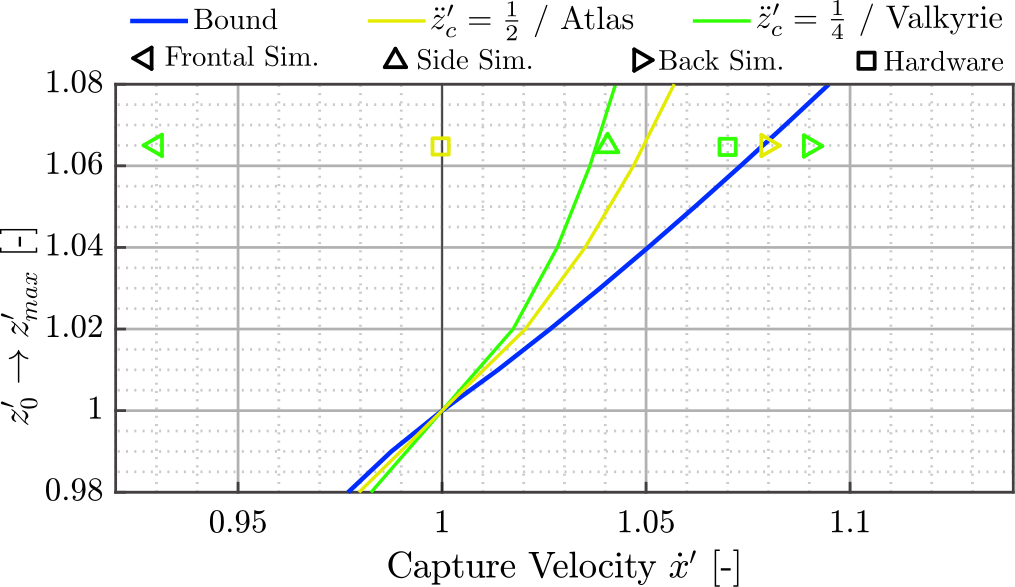
\includegraphics[width=0.9\textwidth]{STYLESTUFF/regioncomparison1.png}
\caption{Difference in recovery of Valkyrie and Atlas in simulation and on hardware between the vertical motion controller and the default setup versus the capture velocity plot of \figref{fig:caplimits}.}
\label{fig:regioncomparison}
\end{figure}

Note how the simulation rear push recovery for Valkyrie even lies outside the height constrained bound in this plot. The average improvement on hardware for Valkyrie lies just inside the height constrained bound. The increase in recovery for the side push in simulation is about equal to the comparable force constrained capture position of $\ddzc'=\frac{1}{4}$. The frontal push recovers worse than the default control setup and is not comparable with the capture regions presented in Chapter \ref{chap:regions}.

\section{Discussion}
In this chapter, a simple control law is presented that activates a bang-bang action if a predefined threshold is met. Using the bang-bang controller, the vertical \ac{CoM} dynamics are explicitly solvable and can be computed every tick. Also, hardware results are presented, which have not earlier been shown considering the research topic. 

A difference between the related works in Section \ref{sec:relatedworksheight} is that most other existing control strategies use \ac{MPC}. With \ac{MPC} however, it all comes down to problem formulation. Caron \& Mallein \cite{caron2018balance} present a method that generates capture trajectories based on the current \ac{CoM} position and velocity, and the support polygon information. The objective is to minimize height variations, which results in the robot to only use vertical \ac{CoM} motion if the desired \ac{ZMP} is placed on the polygon edge. Using this problem formulation though, the resulting capture trajectory is always under the assumption that the previously applied disturbance stopped disturbing. In the case of a push though, the increase in error is not an instant event and happens over time.

The control law in this chapter presents a different approach to the problem. Comparing with the method of \cite{caron2018balance}, which has a constraint on minimum and maximum vertical acceleration in the \ac{MPC} law, the bang-bang controller in this chapter can be seen as the extremum of what the \ac{MPC} would output. Therefore, depending on the selection of the threshold when to activate the controller, the method presented in this chapter will in some cases use more, not necessarily needed, height variation than the control law of \cite{caron2018balance}. However, by using the additional, not necessary, height variations, the method is more robust for longer push durations. The \ac{MPC} law in \cite{caron2018balance} computes capture trajectories based on current velocity differences and does not take expected future disturbances into account.

There are two push recovery test setups considered in this chapter for testing the controller on hardware while the robot is standing. An advantage of the test with the stick is that the force data from the load cell could be measured with an accuracy of $0.25$\% at a record frequency of $100$ [Hz] \cite{iload}. However, many tests had to be conducted to obtain the results of the maximum recoverable pushes, as the person pushing the robot was not always capable of applying the exact same force. With the medicine ball tests, the maximum recoverable push could be found more easily and less tests were needed. However, no measurement data was available of the applied push force. Also, stretch in the rope, a changing \ac{CoM} position in the ball and energy loss of the impact of the ball can all influence the impulse applied on the robot.

Testing push recovery, Valkyrie and Atlas showed a similar behavior in simulation. In \ac{SCS}, a ground stiffness and damping is modeled, where the robot is in contact with the ground with $4$ ground contact points per foot. Also, a joint torque damping is simulated. Therefore, the differences in Atlas and Valkyrie in simulation are predominantly related to the differences in the multi-body structures of the robots.

On hardware however, larger differences were observed when comparing the responses of Valkyrie and Atlas. Valkyrie matched the simulation data with more accuracy, which could be a cause of the torque sensing of the series elastic actuators. However, while performing the tests it is observed that Valkyrie is more sensitive to tuning of the maximum vertical acceleration, maximum jerk and, for example, foot polygon size used in the whole-body \ac{QP}. With careless tuning, Valkyrie could stand on its toes when recovering from a push. Also, the actuators could turn in a state of over-excitation which resulted in the need to restart the robot. Using Atlas, less care had to be taken for tuning and the robot performed well in all tests in terms of internal stability. The less accurate sensing and the stiction in the hydraulic system on Atlas could be a cause that the differences observed between hardware and simulation are larger than on Valkyrie.

To analyze the responses on hardware, phase plots of the horizontal \ac{CoM} state of the robots and different time responses are evaluated. The phase plots give insight in the ability of the robot to return to the desired steady-state configuration. The time response plots show the behavior of momentum rates, joint pitch torques and \ac{CoP} and \ac{ICP} positions over time. However, no traditional system evaluations are conducted, such as a bode plot or other frequency analysis methods. A reason for this is that in the control method, the eigenvalue of the system is time-variant.

On most tests the improvement in recovery of the vertical motion control law versus the default control setup differs  from the difference in the \ac{CP} and the vertical force constraint capture points. Reasons for this could include numerical integration in simulation, unmodeled dynamics such as ground contact or a bug in the software.

Furthermore, the control strategy presented in this chapter is a \ac{2D} strategy. The third dimension is controlled with the $\rcopd$ orthogonal to the push direction, already existing in the control framework. When the robot is walking however, this \ac{2D} strategy does not always improve balance, as the \ac{CoM} is not always in the center of the support polygon if the push is applied. Therefore, the control strategy presented in this chapter is extended in the next chapter for the use while the robot is walking.



